\documentclass[a4paper]{article}
\usepackage[utf8]{inputenc}
\usepackage[ngerman, english]{babel}
\usepackage{mathtools}
\usepackage{amsmath}

\title{\hrule \vspace{0.5cm} AI acceleration on RISC-V using GEMM acceleration cores \vspace{0.5cm} \hrule}
\date{\today, Fürth}
\author{Simon Klier , \and
        Sebastian Fritsch , \and
        Phillip Pelger \and
        and Jan-Niklas Weghorn \\
        \small\textit{Exzellenzcluster Robotik Hardenberg Gymnasium Fürth}
        \thanks{robotik@hardenberg-gymnasium.de}}

\begin{document}

\selectlanguage{ngerman}

\section*{Vorwort}
In diesem Dokument wird unsere Chipidee für den INVENT a CHIP Wettbewerb 2019 vorgestellt.
Wir haben uns entschieden dieses Dokument in englischer Sprache zu verfassen, da unser
Projekt nach Vollendung der Öffentlichkeit kostenfrei bereitgestellt werden soll. Die
Open-Source-Community ist international vertreten und die üblich genutze Sprache ist 
Englisch. Außerdem ist die RISC-V Spezifikation \footnote{https://riscv.org/specifications/}, 
für die wir eine Erweiterung vorschlagen auf Englisch verfasst, weswegen unser Vorschlag
auf Englisch fomuliert ist.

Wir hoffen, dass diese Entscheidung ihnen keine Probleme bereitet. 

\selectlanguage{english}
\maketitle


\twocolumn


\section{Abstract}
Recent breakthroughs in machine learning, especially in the field of multi layer convolutional networks(CNNs) have
led to major improvements in the accuracy, speed and versatility of non-trivial image recognition. However the
execution time on regular CPU architectures has proven to be a major roadblock for the wide adoption of CNN technology. 
We believe that a combination of a energy efficient RISC-V processor and our GEMM
acceleration cores could yield a speed increase of multiple magnitudes while preserving a low energy budget which 
would even allow energy constrained applications like embedded devices to profit of state-of-the-art machine
learning. The RISC-V processor would interface with the acceleration cores through our proposed RISC-V extension.
This would enable hardware manufacturers to change the implementation of their accelerators while keeping compatibility
with older software.

\vspace{0.5cm}
\hrule

\section{Background}

\begin{figure*}[b]
    \centering
    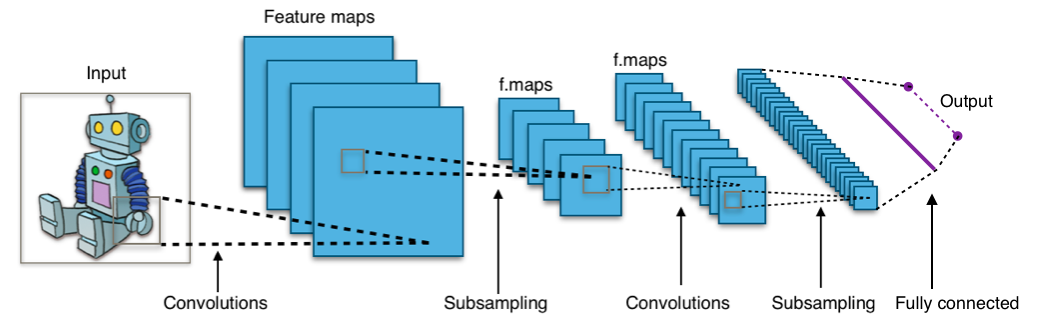
\includegraphics[width=\textwidth]{Typical_cnn.png}
    \caption{Fig.1: Example of a CNN for image classification. Image source: \cite{CNN_example}}
\end{figure*}
\onecolumn



\begin{thebibliography}{99}
\raggedright

\bibitem{CNN_example}
By Aphex34 - Own work, CC BY-SA 4.0, \texttt{https://commons.wikimedia.org/w/index.php?curid=45679374}

\end{thebibliography}



\end{document}
